% LaTeX path to the root directory of the current project, from the directory in which this file resides
% and path to econtexPaths which defines the rest of the paths like \FigDir
\providecommand{\econtexRoot}{}\renewcommand{\econtexRoot}{.}
\providecommand{\econtexPaths}{}\renewcommand{\econtexPaths}{\econtexRoot/Resources/econtexPaths}
% The \commands below are required to allow sharing of the same base code via Github between TeXLive on a local machine and Overleaf (which is a proxy for "a standard distribution of LaTeX").  This is an ugly solution to the requirement that custom LaTeX packages be accessible, and that Overleaf seems to ignore symbolic links (even if they are relative links to valid locations)
\providecommand{\econtex}{\econtexRoot/Resources/texmf-local/tex/latex/econtex}
\providecommand{\econtexSetup}{\econtexRoot/Resources/texmf-local/tex/latex/econtexSetup}
\providecommand{\econtexShortcuts}{\econtexRoot/Resources/texmf-local/tex/latex/econtexShortcuts}
\providecommand{\econtexBibMake}{\econtexRoot/Resources/texmf-local/tex/latex/econtexBibMake}
\providecommand{\econtexBibStyle}{\econtexRoot/Resources/texmf-local/bibtex/bst/econtex}
\providecommand{\econtexBib}{economics}
\providecommand{\notes}{\econtexRoot/Resources/texmf-local/tex/latex/handout}
\providecommand{\handoutSetup}{\econtexRoot/Resources/texmf-local/tex/latex/handoutSetup}
\providecommand{\handoutShortcuts}{\econtexRoot/Resources/texmf-local/tex/latex/handoutShortcuts}
\providecommand{\handoutBibMake}{\econtexRoot/Resources/texmf-local/tex/latex/handoutBibMake}
\providecommand{\handoutBibStyle}{\econtexRoot/Resources/texmf-local/bibtex/bst/handout}

\providecommand{\FigDir}{\econtexRoot/Figures}
\providecommand{\CodeDir}{\econtexRoot/Code}
\providecommand{\DataDir}{\econtexRoot/Data}
\providecommand{\SlideDir}{\econtexRoot/Slides}
\providecommand{\TableDir}{\econtexRoot/Tables}
\providecommand{\ApndxDir}{\econtexRoot/Appendices}

\providecommand{\ResourcesDir}{\econtexRoot/Resources}
\ifnum\pdfshellescape=1
\providecommand{\rootFromOut}{..} % Path back to root directory from output-directory
\providecommand{\LaTeXGenerated}{\econtexRoot/LaTeX} % Put generated files in subdirectory
\providecommand{\EqDir}{\econtexRoot/Equations} % Put generated files in subdirectory
\else
\providecommand{\rootFromOut}{.} % Path back to root directory 
\providecommand{\LaTeXGenerated}{\econtexRoot/} % Put generated files in main directory (because not allowed in subdirectory)
\providecommand{\EqDir}{\econtexRoot/} % Put generated files in main directory
\fi
\providecommand{\econtexPaths}{\econtexRoot/Resources/econtexPaths}
\providecommand{\LaTeXInputs}{\econtexRoot/Resources/LaTeXInputs}

\documentclass[\econtexRoot/BufferStockTheory]{subfiles}
% LaTeX path to the root directory of the current project, from the directory in which this file resides
% and path to econtexPaths which defines the rest of the paths like \FigDir
\providecommand{\econtexRoot}{}\renewcommand{\econtexRoot}{.}
\providecommand{\econtexPaths}{}\renewcommand{\econtexPaths}{\econtexRoot/Resources/econtexPaths}
% The \commands below are required to allow sharing of the same base code via Github between TeXLive on a local machine and Overleaf (which is a proxy for "a standard distribution of LaTeX").  This is an ugly solution to the requirement that custom LaTeX packages be accessible, and that Overleaf seems to ignore symbolic links (even if they are relative links to valid locations)
\providecommand{\econtex}{\econtexRoot/Resources/texmf-local/tex/latex/econtex}
\providecommand{\econtexSetup}{\econtexRoot/Resources/texmf-local/tex/latex/econtexSetup}
\providecommand{\econtexShortcuts}{\econtexRoot/Resources/texmf-local/tex/latex/econtexShortcuts}
\providecommand{\econtexBibMake}{\econtexRoot/Resources/texmf-local/tex/latex/econtexBibMake}
\providecommand{\econtexBibStyle}{\econtexRoot/Resources/texmf-local/bibtex/bst/econtex}
\providecommand{\econtexBib}{economics}
\providecommand{\notes}{\econtexRoot/Resources/texmf-local/tex/latex/handout}
\providecommand{\handoutSetup}{\econtexRoot/Resources/texmf-local/tex/latex/handoutSetup}
\providecommand{\handoutShortcuts}{\econtexRoot/Resources/texmf-local/tex/latex/handoutShortcuts}
\providecommand{\handoutBibMake}{\econtexRoot/Resources/texmf-local/tex/latex/handoutBibMake}
\providecommand{\handoutBibStyle}{\econtexRoot/Resources/texmf-local/bibtex/bst/handout}

\providecommand{\FigDir}{\econtexRoot/Figures}
\providecommand{\CodeDir}{\econtexRoot/Code}
\providecommand{\DataDir}{\econtexRoot/Data}
\providecommand{\SlideDir}{\econtexRoot/Slides}
\providecommand{\TableDir}{\econtexRoot/Tables}
\providecommand{\ApndxDir}{\econtexRoot/Appendices}

\providecommand{\ResourcesDir}{\econtexRoot/Resources}
\ifnum\pdfshellescape=1
\providecommand{\rootFromOut}{..} % Path back to root directory from output-directory
\providecommand{\LaTeXGenerated}{\econtexRoot/LaTeX} % Put generated files in subdirectory
\providecommand{\EqDir}{\econtexRoot/Equations} % Put generated files in subdirectory
\else
\providecommand{\rootFromOut}{.} % Path back to root directory 
\providecommand{\LaTeXGenerated}{\econtexRoot/} % Put generated files in main directory (because not allowed in subdirectory)
\providecommand{\EqDir}{\econtexRoot/} % Put generated files in main directory
\fi
\providecommand{\econtexPaths}{\econtexRoot/Resources/econtexPaths}
\providecommand{\LaTeXInputs}{\econtexRoot/Resources/LaTeXInputs}

\onlyinsubfile{% https://tex.stackexchange.com/questions/463699/proper-reference-numbers-with-subfiles
    \csname @ifpackageloaded\endcsname{xr-hyper}{%
      \externaldocument{\econtexRoot/BufferStockTheory}% xr-hyper in use; optional argument for url of main.pdf for hyperlinks
    }{%
      \externaldocument{main}% xr in use
    }%
    \renewcommand\labelprefix{}%
    % Initialize the counters via the labels belonging to the main document:
    \setcounter{equation}{\numexpr\getrefnumber{\labelprefix eq:AAgg}\relax}% eq:AAgg is the last numbered equation in the main text; start counting up from there
}



\onlyinsubfile{\externaldocument{\LaTeXFiles/BufferStockTheory}} % Get xrefs -- esp to appendix -- from main file; only works properly if main file has already been compiled;
\begin{document}

  \subsection{Diagrams for the Perfect Foresight Model}
  The diagrams below illustrate the order of the several conditions in the text:
  \providecommand{\tikzFigs}{\econtexRoot/Code/LaTeX}
  \medskip
  
  \centerline{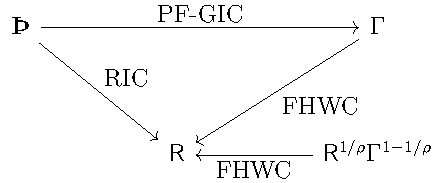
\includegraphics{\tikzFigs/PFGIC-vs-RIC-vs-FHWC}}
% \[
%   \begin{tikzcd}[row sep=large, column sep=large]
%   \textbf{\Thorn} \ar{rr}{\mathrm{\PFGIC}} \ar{dr}{\mathrm{\RIC}}& & \Gamma \ar{dl}{\mathrm{\FHWC}} \\
%    & \mathsf{\Rfree} &
%   \end{tikzcd}
% \]

  and to further incorporate the Perfect Foresight Finite Value of Autarky Condition:
  
  \centerline{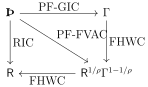
\includegraphics{\tikzFigs/PFGIC-vs-RIC-vs-FHWC-vs-FVAC}}
  
% \[
%   \begin{tikzcd}[row sep=huge, column sep=huge]
%   \textbf{\Thorn} \ar{r}{\mathrm{\PFGIC}} \ar{d}{\mathrm{\RIC}} \ar{dr}{\mathrm{\PFFVAC}}& \Gamma \ar{d}{\mathrm{\FHWC}} \\
%    \mathsf{\Rfree} &  \mathsf{\Rfree}^{1/\CRRA}\Gamma^{1 - 1/\CRRA} \ar{l}{\mathrm{\FHWC}}
%  \end{tikzcd}
%  \]
In both diagrams, an arrow means ``$<$'', which indicates the annotated condition holds, so if a condition is violated, the corresponding arrow is to be reversed. 

These diagrams also keep track of the hierarchy among the conditions. For example, if the right vertical arrow in the second diagram is reversed, then the top right triangle says \PFFVAC + \cncl{\FHWC} implies \PFGIC. If the left vertical arrow is reversed, then \cncl{\RIC} + {\PFGIC} implies \cncl{\FHWC}. 

%\onlyinsubfile{\bibliography{\LaTeXFiles/BufferStockTheory,economics}}


\end{document}
% Local Variables:
% eval: (setq TeX-command-list  (remove '("Biber" "biber %s" TeX-run-Biber nil  (plain-tex-mode latex-mode doctex-mode ams-tex-mode texinfo-mode)  :help "Run Biber") TeX-command-list))
% eval: (setq TeX-command-list  (remove '("Biber" "biber %s" TeX-run-Biber nil  t  :help "Run Biber") TeX-command-list))
% tex-bibtex-command: "bibtex ../LaTeX/*"
% TeX-PDF-mode: t
% TeX-file-line-error: t
% TeX-debug-warnings: t
% LaTeX-command-style: (("" "%(PDF)%(latex) %(file-line-error) %(extraopts) -output-directory=../LaTeX %S%(PDFout)"))
% TeX-source-correlate-mode: t
% TeX-parse-self: t
% eval: (cond ((string-equal system-type "darwin") (progn (setq TeX-view-program-list '(("Skim" "/Applications/Skim.app/Contents/SharedSupport/displayline -b %n ../LaTeX/%o %b"))))))
% TeX-parse-all-errors: t
% End:
